\section{Results}
\label{sec:results}

\subsection{Genetic Correlation}
\label{sub:psych_genetic_correlation}

Foremost, the genetic correlations between impulsive aggression and depressive symptoms is remarkably high ($r_g=0.6741$, $SE=0.0919$, $p=2.2326\times 10^{-13}$).
This high correlation is also reflected in a subjects diagnosed with a major depression ($r_g=0.4134$, $SE=0.1212$, $p=6\times 10^{-04}$).
In contrast, correlations between impulsive aggression and Bipolar disorder did not reached significant levels ($r_g=0.1192$, $SE=0.0949$, $p=0.2091$), and genetic correlations with Schizophrenia, while significant, was not of large effect ($r_g=0.161$, $SE=0.0566$, $p=0.0045$).

In contrast to impulsive aggression, correlations between risk taking and Bipolar ($r_g=0.2561$, $SE=0.0606$, $p=2.4034\times 10^{-05}$), as well as Schizophrenia ($r_g=0.232$, $SE=0.0431$, $p=7.3554\times 10^{-08}$) remain significant after adjusting for multiple testing.
In addition, while genetic correlations were highly significant between aggression and depression, genetic correlations between risk raking, depressive symptoms ($r_g=0.0856$, $SE=0.0687$, $p=0.2129$) as well as MD ($r_g=0.0028$, $SE=0.0853$, $p=0.974$) were small and did not pass the multiple testing threshold.

An overall overview of all genetic correlations are given in Figure~\ref{fig:figures/combined_corr.pdf}.

\begin{figure}[htpb]
  \centering
  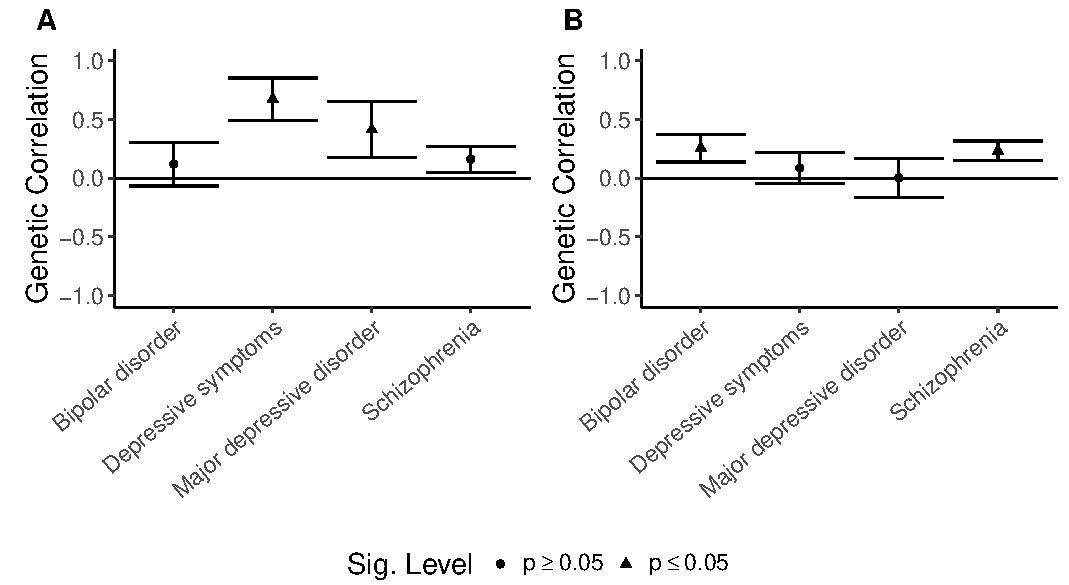
\includegraphics[width=0.8\linewidth]{figures/combined_corr.pdf}
  \caption{Genetic correlations between impulsive aggression and risk taking with selected psychiatric disorders.
    The error bars display the 95\% confidence intervals for each pairwise genetic correlations.
    Significance levels after multiple testing correction are displayed in form of a dot ($p\ge 0.05$) and triangle ($p\leq0.05$).
    (A) Genetic correlations between impulsive aggression and psychiatric disorders. 
    (B) Genetic correlations between risk taking and psychiatric disorders.
  }\label{fig:figures/combined_corr}
\end{figure}


\subsection{Mendelian Randomization}
\label{sub:mendelian_randomization}

Applied MR-methods suggest some indication for a causal effect of depressive symptoms on impulsive aggression (Figure~\ref{fig:overall_mr_effect}).
Specifically, all used method, with the exception of MR-egger support this causal connection.
However, MR Egger, which represents a more conservative approach, displays a different direction of effect.
A possible explanation for this discrepancy can be found in potential pleiotropic effects which might violate MR assumptions.
Inspection of the corresponding funnel plot (see Figure~\ref{fig:sensitivity}) suggest that some pleiotropic effects between selected SNPs and impulsive aggression might be present.

However, a possible causal connection between depression and aggression is further supported by an analysis which includes the summary statistics of the major depressive disorder GWAS\@.
Corresponding to depressive symptoms, while demonstrating smaller effects, this analysis suggests that this sever metal disorder might cause an increase in aggressive behavior. 
Further, all used method suggest the same direction of effect.
Nevertheless, estimates did not reach Significance levels at $\alpha=0.05$.
Inspection of the funnel plot indicates any neglectable pleiotropic effects which might violate underlying assumptions.

\begin{figure}[htpb]
  \centering
  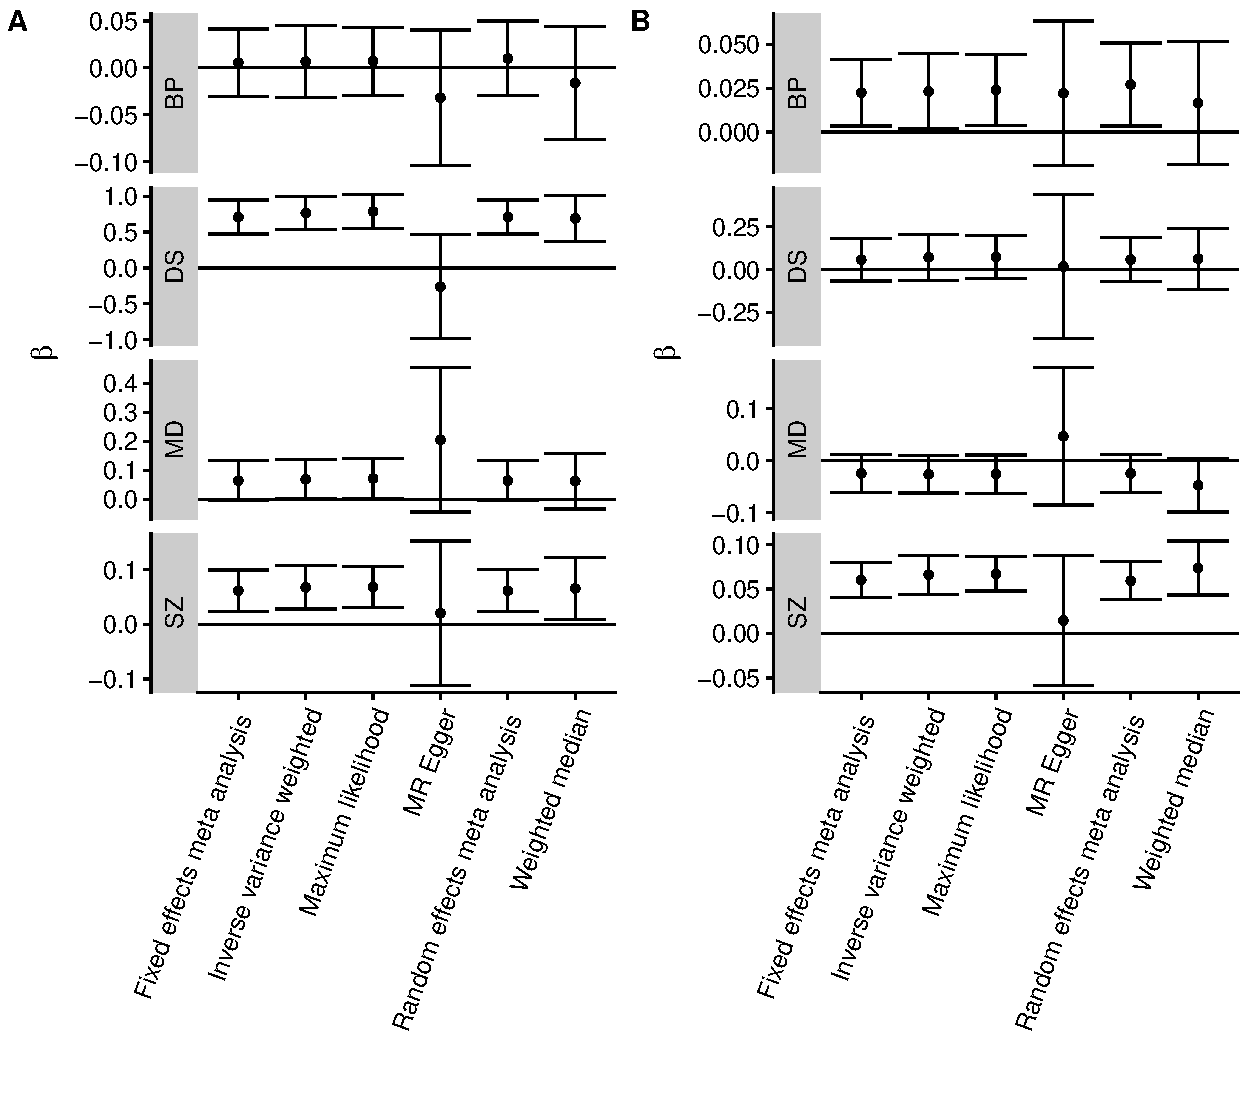
\includegraphics[width=0.9\linewidth]{figures/overall_mr_effect.pdf}
  \caption{Estimated causal effect of psychiatric disorders on impulsive aggression and risk taking.
    The effect size of the causal effect $\beta$ is displayed on the y-axis, while used Mendelian randomization methods are on the x-axis.
    SZ, Schizophrenia; MD, Major Depressive Disorder; DS, Depressive Symptom's; BP, Bipolar Disorder.
    (A) Effect of psychiatric disorders on impulsive aggression.
    (A) Effect of psychiatric disorders on risk taking.
  }\label{fig:overall_mr_effect}
\end{figure}

Further, there is some indication that SZ might cause an increase in aggressive behavior.
Similar to the analyses described above, all but MR-egger suggest a significant effect. 
However, in contrast to the previous described analysis there is very little evidence to support a violation of the underlying MR assumptions.
Thus making a causal connection between these two phenotypes more plausible.

In addition, to aggression MR in connection to risk taking only yield one potential causal relationship.
All used method, with the exception of MR-egger, suggest that Schizophrenia causes an increase in risk taking behavior.
Inspection of both funnel plots and intercept of the MR-egger regression coefficient indicate no major violation of assumptions.

\begin{figure}[htpb]
  \centering
  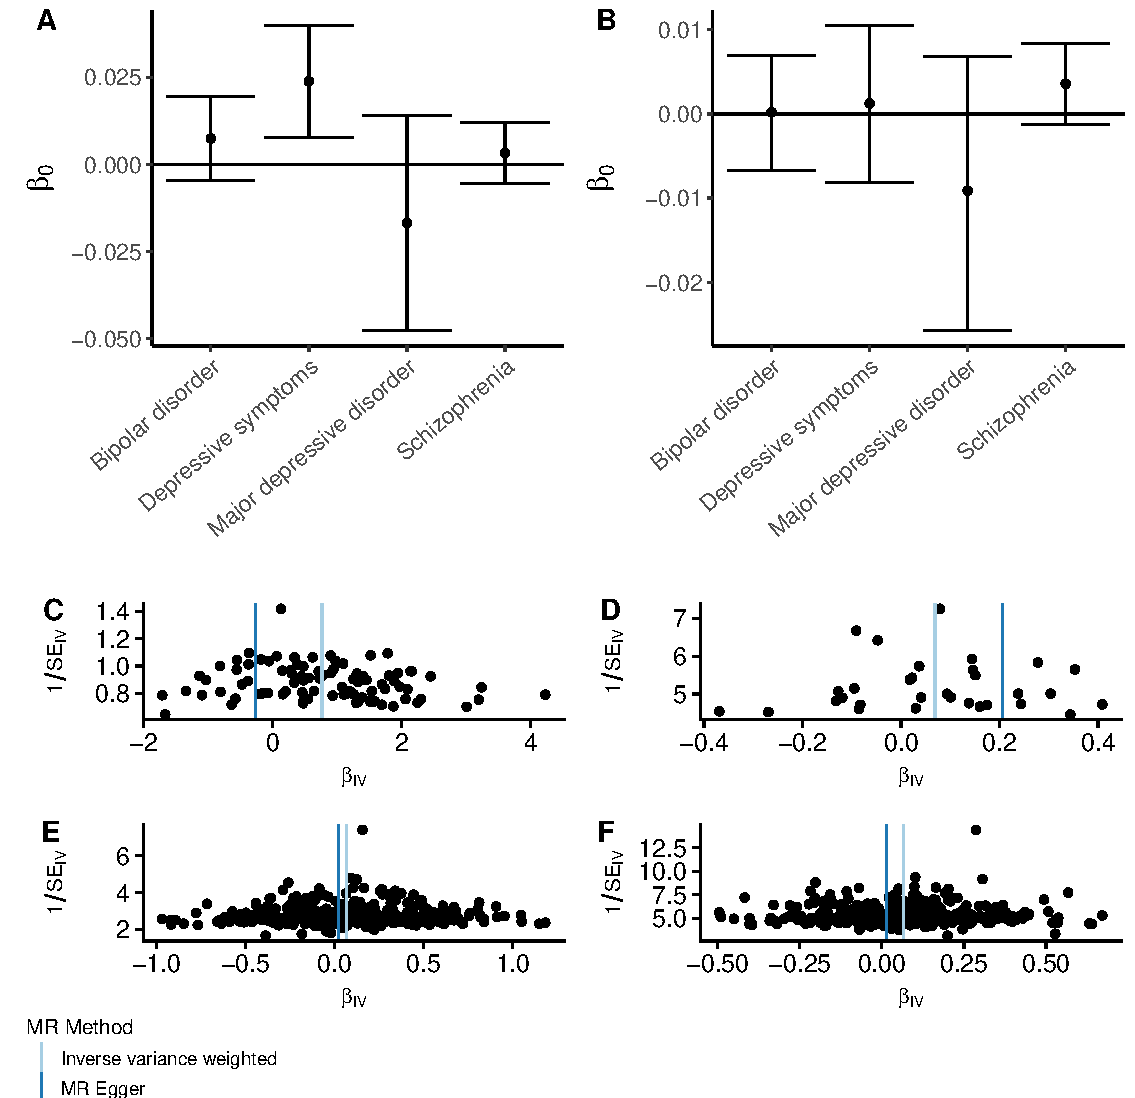
\includegraphics[width=0.9\linewidth]{figures/sensitvity_plot.pdf}
  \caption{Sensitivity analysis.
    (A) Displays the intercept of MR-egger regression for psychiatric disorders on impulsive aggression. The intercept is an indication of whether directional horizontal pleiotropy is driving the MR analysis.
    (B) The MR-egger regression intercept of psychiatric disorders on risk taking.
    (C) Funnel plot of Depressive symptoms on impulsive aggression. 
    (D) Funnel plot of MD on impulsive aggression. 
    (E) Funnel plot of SZ on impulsive aggression. 
    (F) Funnel plot of SZ on risk taking. 
    The intercept of both MR-egger and Inverse variance method are indicated with a vertical line.
    Error bars indicate the 95\% confidence intervals.
  }\label{fig:sensitivity}
\end{figure}

The hypothesised direction between exposure and outcome was tested with the help of the Steiger test~\cite{Steiger1980}.
In general the test examines if the variance explained by the used instrumental SNP in the outcome is less than those within the exposure. 
Careful inspection of these test results suggest that there were no violation of the hypothesised direction of causal effects across all tested connections.

